\section{An\'alsis de FSK y su detector coherente}

Sea la onda FSK
\[ x_c(t)=\sum_k A p_R(t-kT_s)\cos\left(2\pi(f_c+f_k)t\right),\]
donde los pulsos son NRZ de ancho $T_s$ y $f_k=\pm f_\Delta$.

Antes de estudiar el detector, veamos algunas propiedades de la
onda FSK.

\newlength\longUno
\newlength\longDos
\newlength\longitud
\newcommand{\opciones}[2]{%
\settowidth\longUno{#1}%
\settowidth\longDos{#2}%
\ifthenelse{\longUno>\longDos}{\setlength\longitud{1.1\longUno}}{\setlength\longitud{1.1\longDos}}%
\ensuremath{\parbox{\longitud}{\centering \text{#1}\\ \text{#2}}}%
}
\subsection*{Continuidad de fase (entre un símbolo y otro)}
\noindent Suponemos $f_c T_s$ entero, sin pérdida de generalidad.
    En un per\'iodo de símbolo \opciones{$f_k=f_\Delta$}{$f_k=-f_\Delta$}, el cambio de fase es \opciones{$\Delta\phi^+=2\pi f_\Delta T_s$}{$\Delta\phi^-=-2\pi f_\Delta
    T_s$}.

    Para que la onda sea continua, este cambio debe ser igual (a menos de $2\pi m$)
    \begin{gather*}
        \Rightarrow \Delta\phi^+ - \Delta\phi^- = 2m\pi.\\
        \Rightarrow 4 \pi f_\Delta T_s = 2 m \pi \Rightarrow \col{f_\Delta = m \frac{f_s}{2}}
    \end{gather*}
    Visualicemos esto en el caso $f_\Delta=\frac{f_s}{2}$ (FSK de Sunde), con el valor (no
    realista) $f_c=f_s$
    \[\Rightarrow  f_c + f_\Delta = \frac{3}{2}f_s \quad f_c - f_{\Delta} =
    \frac{f_s}{2}.\]

        \begin{center}\begin{minipage}{\textwidth}
        \bpgf{Imagenes/DDPasa/DDPasa-15}
        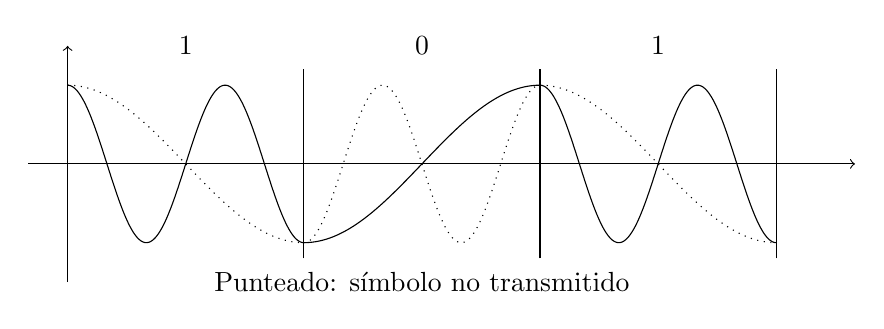
\begin{tikzpicture}
            \draw [->] (-0.5,0) -- (10,0);
            \draw [->] (0,-1.5) -- (0,1.5);
            \draw [domain=0:3,samples=200] plot (\x,{cos(pi*\x r)});
            \draw [domain=0:3,samples=200,dotted] plot (\x,{cos(pi/3*\x r)});
            \draw [domain=3:6,samples=200] plot (\x,{cos(pi/3*\x r)});
            \draw [domain=3:6,samples=200,dotted] plot (\x,{cos(pi*\x r)});
            \draw [domain=6:9,samples=200] plot (\x,{cos(pi*\x r)});
            \draw [domain=6:9,samples=200,dotted] plot (\x,{cos(pi/3*\x r)});
            \draw (3,-1.2) -- (3,1.2);
            \draw (6,-1.2) -- (6,1.2);
            \draw (9,-1.2) -- (9,1.2);
            \path (1.5,1.5) node {$1$} -- (4.5,1.5) node {$0$} -- (7.5,1.5) node {$1$};
            \path (4.5,-1.5) node {Punteado: símbolo no transmitido};
        \end{tikzpicture}
        \endpgfgraphicnamed\end{minipage}
        \end{center}

    \begin{remarkSN}
        Si la fase es continua, esto equivale a la salida de un modulador FM,
        \[A\cos\left(\omega_ct +2\pi f_\Delta \int_{t_0}^t x(\sigma) \d\sigma\right)\]
        cuando la modulante es la onda PAM $x(t)=\sum_k a_k p(t-kT_s)$ con $p(t)=p_{[0,T_s]}(t)$ y $a_k=\pm 1$.
    \end{remarkSN}

    \begin{remarkSN}
        Se puede trabajar con desviación de frecuencia $f_\Delta$ que no cumpla la continuidad de fase, siempre que uno compense estos errores de fase. Este es el caso de MSK (\emph{Minimum Shift Keying}), $f_\Delta=\frac{f_s}{4}$. No entraremos en él.
    \end{remarkSN}

\subsection*{Ortogonalidad de los pulsos}
Calculo el producto
interno de los dos pulsos ($+$ y $-$),
    \begin{align*}
        \frac{1}{T_s}\left<p(t)\cos\left((\omega_c+\omega_\Delta)t\right),p(t)\cos\left((\omega_c-\omega_\Delta)t\right)\right>
        &= \frac{1}{T_s}\int_0^{T_s} \cos\left((\omega_c+\omega_\Delta)t\right)\cos\left((\omega_c-\omega_\Delta)t\right)\d t \\
        & = \frac{1}{2T_s}\int_0^{T_s}\left[\cos(2\omega_\Delta t)+\cos(2\omega_c t)\right]\d t\\
      & \underbrace{=}_{f_c=mf_s} \frac{1}{2T_s} \frac{\sen(2\omega_\Delta T_s)}{2\omega_\Delta} \\
      &=  \frac{1}{2}\sinc(4\pi f_\Delta T_s)=\\
        &= 0 \Leftrightarrow \col{f_\Delta = m\frac{f_s}{4}}
    \end{align*}
    Es menos restrictivo que la continuidad. MSK es el mínimo $f_\Delta$ que cumple la ortogonalidad.

\newpage

\subsection*{Detección FSK coherente}

 \begin{figure}[htb]
    \centering
    \resizebox{\textwidth}{!}{
    \bpgf{Imagenes/DDPasa/DDPasa-16}
    \begin{blockdiagram}
        \matrix[row sep=5mm, column sep=10mm,ampersand replacement=\&]{
            \& \& \& \& \& \&\node[operator] (mult1) {$\times$}; \& \node[block] (int1) {$\frac{1}{T_s}\int_{t-T_s}^t$};\\
            \node[punto] (inicio) {}; \& \& \& \& \& \node [punto] (p) {}; \& \node[etiqueta] (osc1) {$2\cos\left((\omega_c+\omega_\Delta)t\right)$}; \& \& \&\node[operator] (sum) {} node [anchor=north east] {$-$} node [anchor=south east] {$+$}; \& \node [block] (comp) {COMP.};\\
            \& \& \& \& \& \&\node[operator] (mult2) {$\times$}; \& \node[block] (int2) {$\frac{1}{T_s}\int_{t-T_s}^t$};\\
            \& \& \& \& \& \&\node [etiqueta] (osc2) {$2\cos\left((\omega_c-\omega_\Delta)t\right)$};\\
        };
        \draw (inicio) -- node [anchor=south] {$A\cos\left((\omega_c\pm\omega_\Delta)t\right)+n(t)$} node [anchor=north] {$S_n(f)=\frac{\eta}{2}$ en la banda} (p);
        \draw [->] (p) |- (mult1);
        \draw [->] (osc1) -- (mult1);
        \draw [->] (mult1) -- (int1);
        \draw [->] (int1) -| node [anchor=west] {$z^+$} (sum);
        \draw [->] (p) |- (mult2);
        \draw [->] (osc2) -- (mult2);
        \draw [->] (mult2) -- (int2);
        \draw [->] (int2) -| node [anchor=west] {$z^-$} (sum);
        \draw [->] (sum) -- (comp);
    \end{blockdiagram}
    \endpgfgraphicnamed}
 \end{figure}
 \FloatBarrier

 \paragraph{Idea:} calculo ambos productos internos en un período de símbolo, según cual sea
 mayor se toma la decisión de detección.

Analicemos el caso en que se recibió el símbolo $f_c+f_\Delta$ (el
otro es análogo).
    \begin{align*}
        z^+(T_s) &= \frac{2}{T_s} \left<A p(t) \cos\left((\omega_c+\omega_\Delta)t\right)+n(t),\cos\left((\omega_c+\omega_\Delta)t\right)\right>\\
        &= \frac{2A}{T_s} \left\|p(t)\cos\left((\omega_c+\omega_\Delta)t\right)\right\|^2 +
        \frac{2}{T_s}\left<n(t),p(t)\cos\left((\omega_c+\omega_\Delta)t\right)\right>\\
        & =A+n^+.
     \end{align*}
Aquí usamos que la norma del primer término es $\frac{T_s}{2}$.
%por lo tanto obtenemos
%    \[\col{z^+(T_s)=}\]
    \begin{align*}
        z^-(T_s) &= \frac{2A}{T_s}\left<p(t)\cos\left((\omega_c+\omega_\Delta)t\right),p(t)\cos\left((\omega_c-\omega_\Delta)t\right)\right>  + \frac{2}{T_s}\left<n(t),p(t)\cos\left((\omega_c-\omega_\Delta)t\right)\right>\\
        &= A\sinc(4\pi f_\Delta T_s) + n^-\\
        &= n^- \rightarrow \text{si los pulsos son ortogonales.}
    \end{align*}
   \begin{remarkSN}
    Mejor que la ortogonalidad sería que el producto interno (el
    sinc) fuese negativo.  Se trabaja en general con pulsos ortogonales, lo cual
    asumimos.\vspace{-0.5cm}
    \end{remarkSN}
    \[\col{z^+(T_s)-z^-(T_s) = A + n^+ - n^-}\]

    Comparando con el umbral $0$, cometo un error si  $A + n^+ - n^- < 0  \Leftrightarrow n^- -
    n^+ > A$.
    \[\Rightarrow P_e = Q\left(\frac{A}{\sigma}\right), \text{ donde } \sigma^2 = E\left[(n^- - n^+)^2\right].\]

    \begin{align*}
        n^- - n^+ &= \frac{2}{T_s} \int_0^{T_s} n(t)\left[\cos\left((\omega_c - \omega_\Delta)t\right) - \cos\left((\omega_c + \omega_\Delta)t\right)\right]\d t\\
        &= \frac{4}{T_s} \int_0^{T_s} n(t)\sen(\omega_c t)\sen(\omega_\Delta t)\d
        t.
    \end{align*}

    Para calcular $\sigma^2$, pensar en un filtro de respuesta impulsiva $h(t)$, con
    \[h(T_s-t)=\frac{1}{T_s} p(t) 4 \sen(\omega_c t)\sen(\omega_\Delta t)\]
    excitado por ruido blanco $(\frac{\eta}{2})$.  Entonces $n^- - n^+ = (h\ast
    n)\big|_{t=T_s}$.
    \[\Rightarrow E\left[(n^- - n^+)^2\right] = \frac{\eta}{2} \int_{-\infty}^{+\infty} |\hat{H}(f)|^2 \d f= \frac{\eta}{2} \|h\|^2 = \frac{\eta}{2T_s^2} \int_0^{T_s} 16 \sen^2(\omega_c t)\sen^2(\omega_\Delta t)\d t.\]
    Como $\sen^2(\omega_c t)$ var\'ia muy rápido, lo aproximo por su valor medio
    $\frac{1}{2}$.
    \begin{align*}
        \Rightarrow \sigma^2 &= \frac{\eta}{2T_s^2}8\int_0^{T_s}\sen^2(\omega_\Delta t)\d t\\
        &= \frac{4\eta}{T_s^2} \int_0^{T_S}\left[\frac{1}{2} - \frac{\cos(2\omega_\Delta t)}{2}\right]\d t\\
        &= \frac{2\eta}{T_s} \left[1 - \sinc(2\omega_\Delta
        T_s)\right].
    \end{align*}
    Suponiendo la condición de ortogonalidad de pulsos, obtenemos
    $\col{\sigma^2 = 2\eta f_s}$

    Aquí la energía del pulso es $\frac{A^2}{2} T_s = \overline{E_p} \Rightarrow \col{A^2 = 2\overline{E_p} f_s}$
    \[\Rightarrow \frac{A}{\sigma} = \sqrt{\frac{\overline{E_p}}{\eta}} \Rightarrow \col{P_e=Q\left(\sqrt{\frac{\overline{E_p}}{\eta}}\right)}\]
    igual que ASK, igual que unipolar banda base.


\subsection*{Recapitulando (detección coherente)}

Mediante correlación y comparación con umbrales puedo detectar
ASK, BPSK, BFSK con performance similar. También QAM, M-PSK de más
eficiencia espectral. Es común representar este desempeño en
términos de una gráfica de $P_e$, en escala logar\'itmica, en
funci\'on de $\frac{\overline{E_p}}{\eta}$ en dB.



\begin{figure}[htb]
    \centering\begin{minipage}{\textwidth}
    \bpgf{Imagenes/DDPasa/DDPasa-17}
    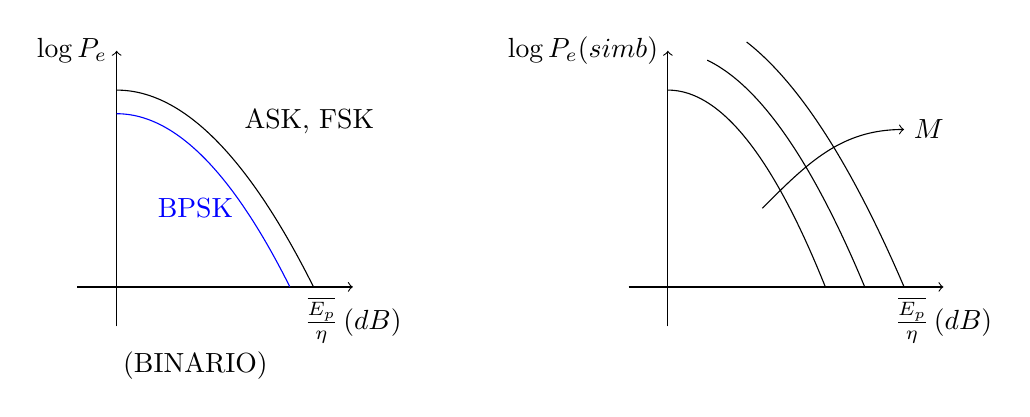
\begin{tikzpicture}
        \draw [->] (-0.5,0) -- (3,0) node [anchor=north] {$\frac{\overline{E_p}}{\eta}\,(dB)$};
        \draw [->] (0,-0.5) -- (0,3) node [anchor=east] {$\log P_e$};
        \draw [domain=0:2.2,samples=200,blue] plot (\x,{2.2 - (\x^2/2.2)});
        \path [blue] (1,{2.2-1/2.2-0.5}) node [anchor=north]{BPSK};
        \draw [domain=0:2.5,samples=200,] plot (\x,{2.5 - (\x^2)/2.5});
        \path (1.5,{2.5-1/2.5}) [anchor=west] node{ASK, FSK};
        \path (1,-1) node {(BINARIO)};
 %       \path (2.5,1) node [anchor=west] {\parbox{3cm}{curva depende (no mucho) de modul.}};

        \begin{scope}[shift={(7,0)}]
            \draw [->] (-0.5,0) -- (3.5,0) node [anchor=north] {$\frac{\overline{E_p}}{\eta}\,(dB)$};
            \draw [->] (0,-0.5) -- (0,3) node [anchor=east] {$\log P_e(simb)$};
            \draw [domain=0:2,samples=200,] plot (\x,{2.5 - 2.5/4*(\x^2)});
            \draw [domain=0.5:2.5,samples=200,] plot (\x,{3 - 3/2.5^2*(\x^2)});
            \draw [domain=1:3,samples=200,] plot (\x,{3.5 - 3.5/3^2*(\x^2)});
            \draw [->] (1.2,1) [out=45,in=180] to (3,2) node [anchor=west] {$M$};
        \end{scope}
    \end{tikzpicture}
    \endpgfgraphicnamed\end{minipage}
\end{figure}
